\newSec{Regelsysteme}{1}

In der Norm \textit{DIN IEC 60050-351} (\textit{Internationales Elektrotechnisches Wörterbuch – Teil 351: Leittechnik}), welche Begriffe der Regelungstechnik definiert, wird der Begriff \textit{Regelung} wie folgt beschrieben: \cite{IEC60050-351}\\
\glqq Vorgang, bei dem fortlaufend eine variable Größe, die Regelgröße, erfasst, mit einer anderen variablen Größe, der Führungsgröße, verglichen und im Sinne einer Angleichung an die Führungsgröße beeinflusst wird.\\\note{Kennzeichen für das Regeln ist der geschlossene Wirkungsablauf, bei dem die Regelgröße im
Wirkungsweg des Regelkreises fortlaufend sich selbst beeinflusst.}\grqq 


In diesem Kapitel sollen regelungstechnische Grundlagen beschrieben werden.





\newSec{Regelkreis}{2}

Im Allgemeinen grenzen sich die Konzepte \textit{steuern} und \textit{regeln} durch die Eigenschaft der Rückkopplung des Systems ab. Gesteuerte Systeme wirken lediglich auf Aktoren, wobei geregelte Systeme die Abweichung des \textit{Ist}-Zustandes vom \textit{Soll}-Zustand ermitteln und eine geeignete Veränderung erzielen sollen.\comp{IEC60050-351}




\begin{figure}[ht!]
\vspace{0.25cm}
\begin{center}
\fbox{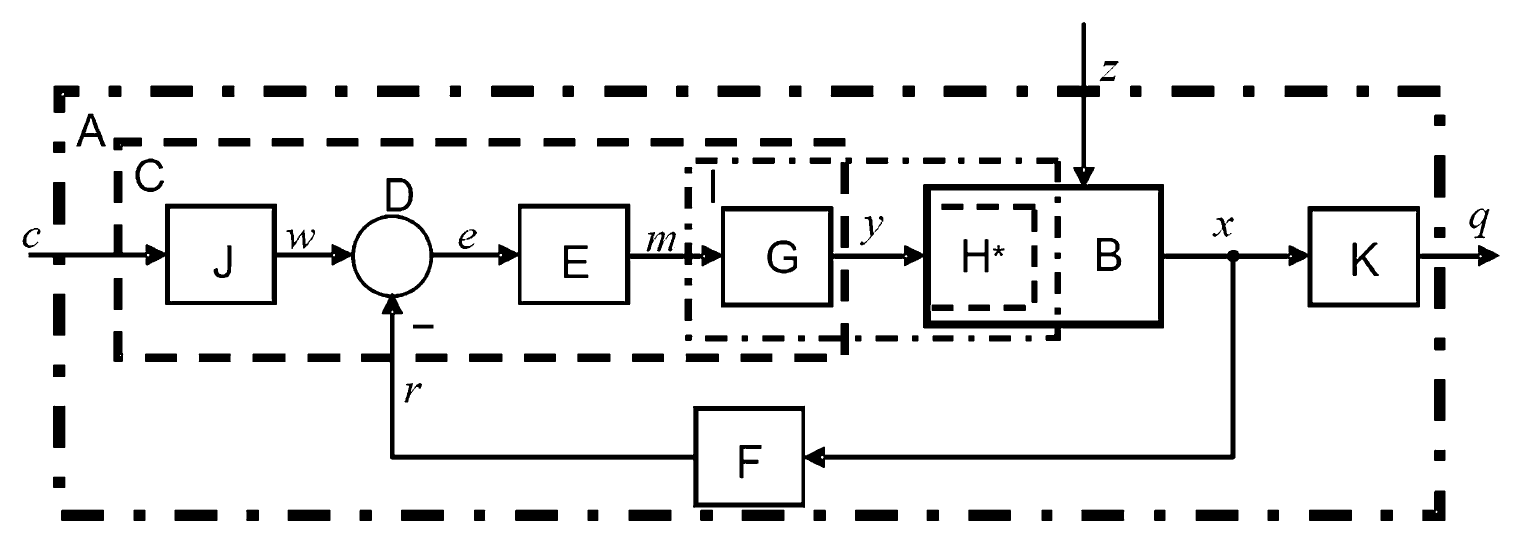
\includegraphics[width=15cm]{Pictures/Control Schema.png}}

\begin{tabular}{ll|ll}
	A  & Regelungssystem       & K & Bildung der Aufgabengröße \\
	B  & Regelstrecke          & c & Zielgröße                 \\
	C  & Regeleinrichtung      & w & Führungsgröße             \\
	D  & Vergleichsglied       & e & Regeldifferenz            \\
	E  & Regelglied            & m & Reglerausgangsgröße       \\
	F  & Messglied             & y & Stellgröße                \\
	G  & Steller               & z & Störgröße                 \\
	H* & Stellglied            & x & Regelgröße                \\
	I  & Stelleinrichtung      & q & Aufgabengröße             \\
	J  & Führungsgrößenbildner & r & Rückführgröße            
\end{tabular}
\caption{Allgeimeines Schema eines Regelkreises \cite{IEC60050-351}}
\label{fig:Contr}
\end{center}
\vspace{0.25cm}
\refImgShort{fig:Contr} zeigt \missing\
\end{figure}









\newSec[Regelerarten]{Arten von Reglern}{2}



\newSec[ControlP]{P-Regler}{3}



\newSec[ControlI]{I-Regler}{3}



\newSec[ControlD]{D-Regler}{3}



\newSec[ControlPID]{PID-Regler}{3}



\newSec[ControlPT]{PT-Regler}{3}

\missing[Dient der Abbildung realer Systeme, welche sich an einen Zustand anpassen müssen. Drehzahlen, Temperaturen etc.]




\newSec{Stabilität}{2}


\missing[nur anmerken, dass es Instabile Systeme gibt => Bode-Diagramm nennen]

